
\documentclass[ms.tex]{subfiles} 
\begin{document} 

\section{Results} 
\label{sec:results} 

\subsection{The Fiducial Model} 
\label{sec:results:fiducial} 

\begin{figure*} 
\centering 
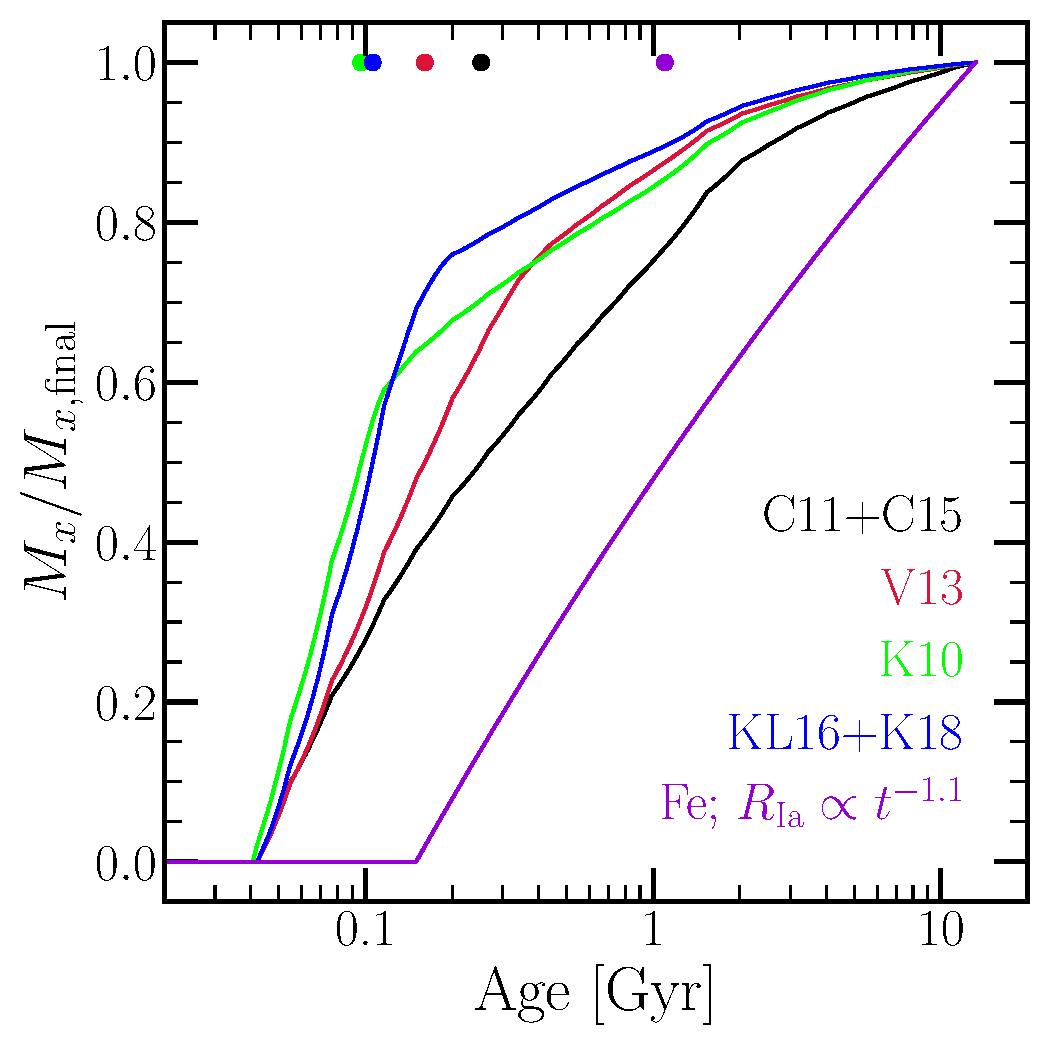
\includegraphics[scale = 0.45]{ssp_production_modelcomp.pdf} 
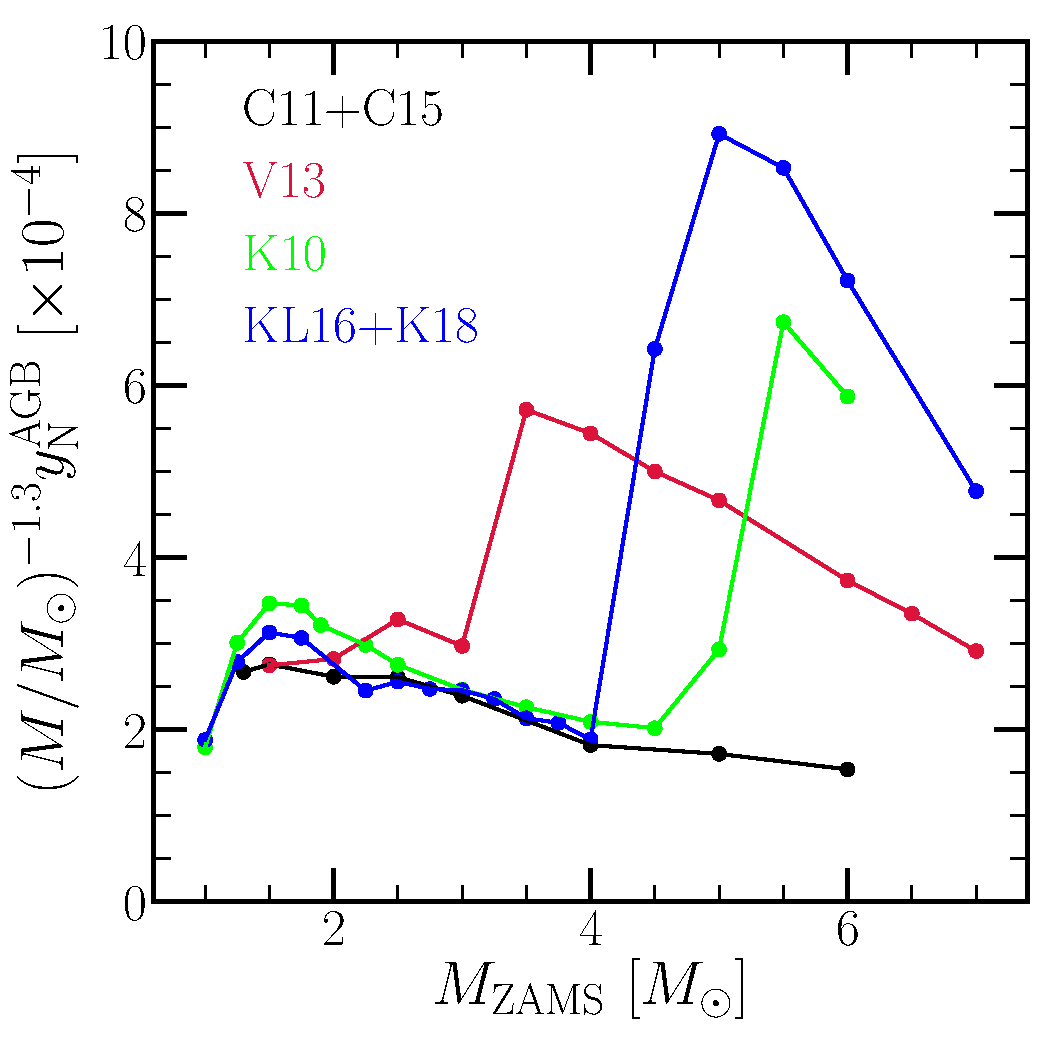
\includegraphics[scale = 0.45]{agb_yield_models_imfweighted.pdf} 
\caption{ 
\textbf{Left}: The net mass of N produced by AGB stars from a single stellar 
population for each of our yield models at solar metallicity 
($Z = 0.02$ in~\karakasten,~$Z = 0.014$ otherwise). 
The purple line denotes the same for Fe assuming our~$t^{-1.1}$ delay time 
distribution. 
All values are normalized to the total mass produced at an age of 13.2 Gyr. 
Points at the top of the panel denote the ages at which 50\% of the total mass 
yield has been produced. 
\textbf{Right}: The IMF-weighted mass yield of N from AGB stars as a function 
of progenitor mass at the same metallicities as in the left panel. 
} 
\label{fig:ssp} 
\end{figure*} 

\begin{itemize} 
	\item Our fiducial model adopts, together with the supernova yields 
	of~\citet[][see discussion in~\S~\ref{sec:methods}]{Johnson2021}, 
	$y_\text{N}^\text{CC} = 3.6\times10^{-4}$ and the~\cristallo~AGB star yield 
	tables. 

	\item To obtain the [N/O]-[O/H] relation predicted by the model, we simply 
	take the N and O abundances in the gas-phase at a given time for 
	each~$\delta\rgal$ = 100 pc ring at~$\rgal >$ 2 kpc and plot them as a 
	line.
	We show the results at five output times in the left hand panel of 
	Fig.~\ref{fig:no_oh_timeevol}. 
	The relation is generally time-independent after~$T \gtrsim 5$ Gyr, though 
	there is some evolution toward higher [N/O]. 

	\item The small bumpy features in the relation are caused by stellar 
	migration; in comparison, the dotted lines plotted at~$T = 2$ and 5 Gyr 
	quantify the prediction when migration is neglected (i.e. the 
	``post-processing'' model from~\citealt{Johnson2021}). 
	At a given time, the movements of stars between rings induce a slight 
	surplus or deficit in the number of AGB stars enriching some annulus. 
	This is similar to what~\citet{Johnson2021} found for SN Ia enrichment of 
	Fe (see discussion in their~\S\S~3.2 and 3.4). 
	Generally the effect is small for N ($<$0.1 dex), but there are some 
	instances at early times where the impact of stellar migration is more 
	substantial. \tabularnewline
	
	\item In our models, the [N/O]-[O/H] relation arises as a superposition of 
	endpoints rather than an evolutionary phase. 
	We demonstrate this in the middle panel of 
	Fig.~\ref{fig:no_oh_timeevol}, where we plot the time-evolution of 
	[N/O] and [O/H] at~$\rgal = 4$, 6, 8, 10, and 12 kpc in relation to the 
	predicted [N/O]-[O/H] relation at the present day. 
	Rather than each annulus's track passing through some well-defined region 
	of this parameter space, they instead each evolve upward more or less 
	parallel to one another. 
	The result is an [N/O]-[O/H] relation that reflects the Galaxy's 
	metallicity gradient more so than different evolutionary states. 
	Similar arguments have been made regarding the low [$\alpha$/Fe] stars in 
	the Galaxy~\citep[see, e.g.,][]{Schoenrich2009, Sharma2020}. 
\end{itemize} 

\subsection{Alternate Yield Models} 
\label{sec:results:yields} 

\begin{figure*} 
\centering 
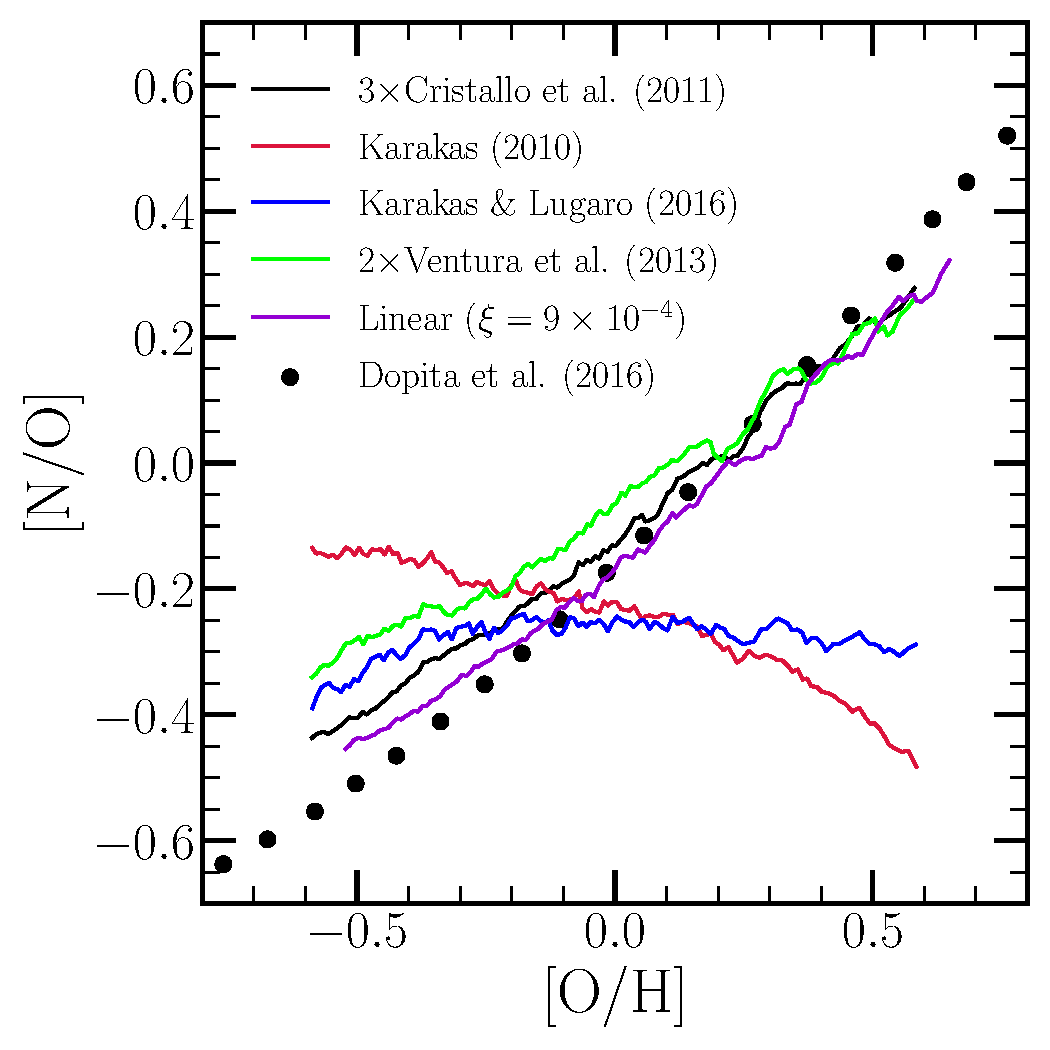
\includegraphics[scale = 0.45]{no_oh_predictions.pdf} 
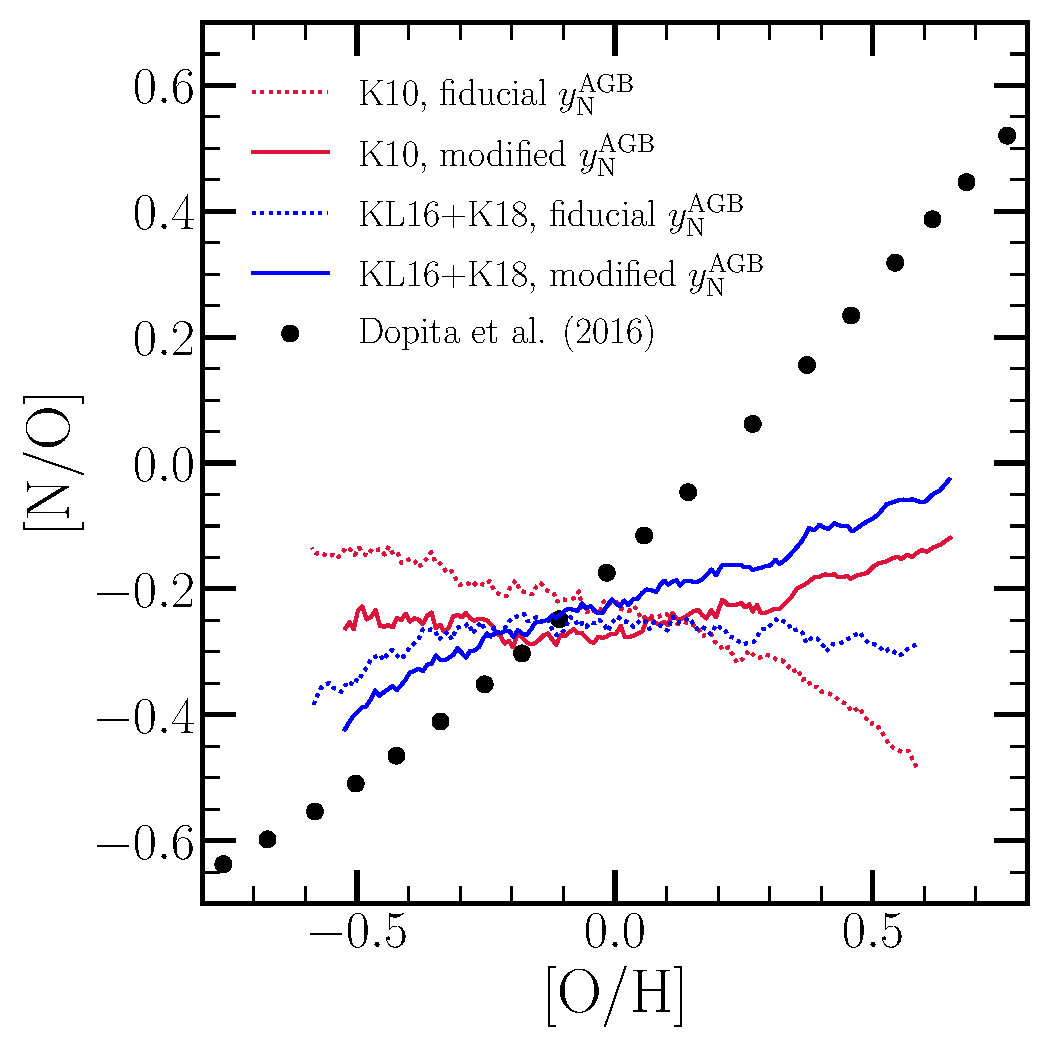
\includegraphics[scale = 0.45]{no_oh_predictions_karakas.pdf} 
\caption{
\textbf{Left}: The present day gas-phase [N/O]-[O/H] relation predicted by our 
fiducial model with each of the yield sets described 
in~\S~\ref{sec:methods:agb}. 
The~\cristallo~and~\ventura~yields are artificially amplified by factors of 
3 and 2, respectively, and we take the linear model with~$\xi = 9\times10^{-4}$. 
For observational reference, we plot the population-averaged trend for local 
stars and HII regions reported by~\citet{Dopita2016}. 
\textbf{Right}: The same as the left-hand panel, but comparing the predictions 
made by the~\karakasten~and~\karakas~yields with our fiducial value 
of~$y_\text{N}^\text{CC}$ (dotted lines, same as left-hand panel) to those with 
the alternate forms of~$y_\text{N}^\text{CC}$ (solid lines) given by equation X 
for the~\karakasten~yields and equation Y for the~\karakas~yields. 
} 
\label{fig:no_oh_predictions} 
\end{figure*} 

\begin{itemize} 
	\item The smaller impact of stellar migration on N than Fe abundances can 
	be understood by their timescales for production from single stellar 
	populations. 
	To demonstrate this, we make use 
	of~\vice's~\texttt{vice.single\_stellar\_population} function, which 
	computes the mass yield of a given element as a function of time from a 
	star cluster of known metallicity. 
	For the sake of this calculation, we set~$y_\text{N}^\text{CC}$ and 
	$y_\text{Fe}^\text{CC}$ both to zero in order to highlight only the 
	delayed nucleosynthetic sources. 
	We plot the results of this procedure in the left panel of 
	Fig.~\ref{fig:ssp} for each of our AGB star yield models at solar 
	metallicity ($Z = 0.02$ for~\karakasten,~$Z = 0.014$ otherwise). 
	Under our fiducial model, it takes~$\sim$250 Myr for a single stellar 
	population to produce~$\sim$50\% of its N from AGB stars. 
	For Fe, this characteristic delay time is near~$\sim$1 Gyr, an order of 
	magnitude larger.\footnote{
		This is exactly as expected with a~$\sim t^{-1}$ DTD as adopted 
		in~\citet{Johnson2021}. 
		Half of the SNe Ia occur between 100 Myr and 1 Gyr, and the other half 
		between 1 and 10 Gyr. 
	} 
	\citet{Johnson2021} find that the Fe enrichment rate can vary by as much 
	as a factor of~$\sim$3 due only to stellar migration (see their Fig. 8 and 
	discussion in their~\S~3.4). 
	This is largely because the timescales for migration are comparable to the 
	timescales for SN Ia explosions, but the same is not true for N. 
	Instead, N is produced on shorter timescales, meaning that single stellar 
	populations generally eject most of their yield to the ISM before their 
	orbits can change significantly. 
	\begin{itemize} 
		\item Despite minor differences in the details of the predicted delay 
		time distributions, there is good qualitative agreement between our 
		different AGB star yield models. 
		Our fiducial model with~\cristallo~yields is the slowest, owing to the 
		larger N production in~$\gtrsim3\ \msun$ stars in the alternate 
		models. 
		As a consequence, the alternate models predict even less variability 
		in the gas phase N abundances due to stellar migration. 
	\end{itemize} 

	\item In the right hand panel of Fig.~\ref{fig:ssp}, we plot the 
	IMF-weighted mass yield of nitrogen for each of our yield models at the 
	same metallicities as in the left hand panel. 
	Since our yields are fractional (or rather, in units of the progenitor 
	star's mass; see discussion in~\S~\ref{sec:methods:agb}), the mass 
	yield is given by M$y_\text{N}^\text{AGB}$. 
	With an additional weight of M$^{-2.3}$ from the IMF in this mass 
	range~\citep{Kroupa2001}, we thus multiply each yield 
	by (M$/\msun)^{-1.3}$. 
	Compared to the fiducial model, the contribution of higher mass AGB stars 
	to the total N production is quite substantial. 
	The difference can be understood by the interaction between TDU and HBB 
	discussed in~\S~\ref{sec:methods:agb} which effects the evolution 
	of stars at these masses. 

	\item The left hand panel of Fig.~\ref{fig:no_oh_predictions} compares the 
	predictions of our model made with each of the AGB star yield models 
	discussed in~\S~\ref{sec:methods:agb} and visualized in 
	Fig.~\ref{fig:agb_yield_models}. 
	For observational reference, we include the~\citet{Dopita2016} measurements 
	also plotted in Fig.~\ref{fig:no_oh_observed}. 

	\item In order to successfully reproduce the observations, we find that we 
	need to artificially amplify the~\cristallo~and~\ventura~yields by factors 
	of~$\sim$3 and~$\sim$2, respectively. 
	Having originally comparing our linear model to the~\cristallo~yields in 
	Fig.~\ref{fig:agb_yield_models} with~$\xi = 3\times10^{-4}$, we amplify the 
	value of~$\xi$ by a factor of 3 here as well. 
	Although these models predict an [N/O]-[O/H] relation that is slightly 
	shallower than the~\citet{Dopita2016} measurements, the predictions are 
	reasonably within the scatter seen in Fig.~\ref{fig:no_oh_observed}. 
	{\color{red} To do: Alternatively, can this be explained by a lowering of 
	the O yields and~$\eta$, or a differential wind which preferentially 
	removes oxygen~\citep{Vincenzo2016}}? 

	\item We are unable to reproduce the observed trend with either 
	the~\karakasten~or~\karakas~yield models. 
	\begin{itemize} 
		\item In the case of~\karakasten, the model overpredicts [N/O] at low 
		[O/H] and predicts [N/O] to~\textit{decrease} monotonically with 
		increasing [O/H]. 
		With a slope of the wrong sign, there is no multiplicative factor by 
		which we can amplify or suppress these yields in order to reproduce the 
		observations. 

		\item The~\karakas~yields improve upon the~\karakasten~predictions to 
		some extent. 
		The overprediction of [N/O] at low [O/H] is largely corrected, but it 
		predicts a relatively flat trend of [N/O] above [O/H]~$\gtrsim -0.2$, 
		leading still to an underprediction of [N/O] at high [O/H]. 
	\end{itemize} 

	\item Can an alternate parameterization of~$y_\text{N}^\text{CC}$ reproduce 
	the observations with the~\karakasten~and~\karakas~AGB star yield models? 
	\begin{itemize} 
		\item If the~\karakasten~yields are to reproduce the observations, the 
		overall N abundance must decrease at low [O/H] and increase at high 
		[O/H]; one way to do this is with a metallicity-dependent CCSN yield. 
		We therefore construct the following parameterization 
		of~$y_\text{N}^\text{CC}$: 
		\begin{equation} 
		y_\text{N}^\text{CC} = (3.6\times10^{-4})\left(\frac{Z}{Z_\odot}\right). 
		\label{eq:linear_yncc} 
		\end{equation} 
		We illustrate this model with the slanted black dotted in 
		Fig.~\ref{fig:n_cc_yields}. 
		While our fiducial model best describes the rotating CCSN models 
		of~\citet{Limongi2018}, this alternate parameterization better 
		characterizes the non-rotating models of~\citet{Limongi2018}, 
		\citet{Sukhbold2016}, \citet{Nomoto2013}, and~\citet{Woosley1995} while 
		maintaining the same base-line value of~$3.6\times10^{-4}$ at solar 
		metallicity. 

		\item If the~\karakas~yields are to reproduce the observed results, 
		then contrary to the predictions made with the~\karakasten~yields, the 
		overall N abundance at low [O/H] is fine. 
		Instead, it's only the N abundance at high [O/H] that needs 
		correcting. 
		We therefore construct a second alternate form of~$y_\text{N}^\text{CC}$ 
		by retaining the value of the fiducial yield at sub-solar metallicity 
		but assuming the value of equation~\refp{eq:linear_yncc} above solar 
		metallicity: 
		\begin{equation} 
		y_\text{N}^\text{CC} = \begin{cases} 
		3.6\times10^{-4} & (Z \leq Z_\odot) 
		\\ 
		(3.6\times10^{-4})\left(\frac{Z}{Z_\odot}\right) & (Z \geq Z_\odot). 
		\end{cases} 
		\label{eq:broken_yncc} 
		\end{equation} 

		\item We compare our model predictions with these alternate CCSN yields 
		for the~\karakasten~and~\karakas~AGB star yields in the right hand 
		panel of Fig.~\ref{fig:no_oh_predictions}. 
		These modifications were able to make up some of the difference, but 
		both models still predict an [N/O]-[O/H] relation that is simply too 
		shallow to explain the observations. 
		Although we cannot reproduce the data with either the~\karakasten~or 
		\karakas~yield models, they suffer from similar issues as 
		the~\cristallo~and~\ventura~yields. 
		\begin{itemize} 
			\item The underprediction of N yields at high metallicity is not 
			unique to~\karakasten~and~\karakas; we have to amplify 
			the~\cristallo~and~\ventura~yields by factors of a few for this 
			exact reason. 

			\item At low [O/H], the~\karakas~yields are actually the only ones 
			that can explain the observed N abundances without any 
			modification. 
			The~\karakasten~yields, however, overpredict the N abundances at 
			low metallicity. 

			\item The inverse dependence of [N/O] with [O/H] when taking 
			the~\karakasten~yields can be understood by the interaction between 
			TDU and HBB (see discussion in~\S~\ref{sec:methods:agb}). 
			Both effects are stronger at low metallicity, and since all of 
			the~\karakasten~models experiencing HBB also experience TDU (see 
			their Table 1), such a result is not surprising. 
			This is also true for the~\karakas~yields, but that model predicts 
			a relatively flat [N/O]-[O/H] relation. 
			
			\item We cannot say with any confidence based on our GCE models 
			whether or not such a wide mass range of stars should experience 
			both TDU and HBB. 
			On the one hand, this makes it difficult for the model to predict a 
			monotonic increase in [N/O] with increasing [O/H]. 
			On the other hand, such strong N production at low metallicity in 
			the~\karakas~yields is what allows them to explain the N abundances 
			at low [O/H] with no modification. 
		\end{itemize} 

		\item We believe these results are independent of the choice of the 
		CCSN yield of O~$y_\text{O}^\text{CC}$. 
		Our value of~$y_\text{O}^\text{CC}$ = 0.015 is based on models in which 
		all stars with a ZAMS mass above 8~\msun~explode as a 
		CCSN~\citep[e.g.][]{Chieffi2013}, but the~\citet{Johnson2021} models 
		assume substantial outflows such that the equilibrium abundance 
		corresponds to a reasonable metallicity gradient within the Galaxy. 
		If we were to lower all of our CCSN yields by a factor of 3 to account 
		for failed supernovae~\citep[e.g.][]{Sukhbold2016}, then we would have 
		to also lower our mass loading factors by a factor of 3 to predict 
		similar overall abundances~\citep{Weinberg2017}. 
		Our model would thus compute similar AGB star yields for N in such a 
		scenario. 

	\end{itemize} 
\end{itemize} 

\begin{figure*} 
\centering 
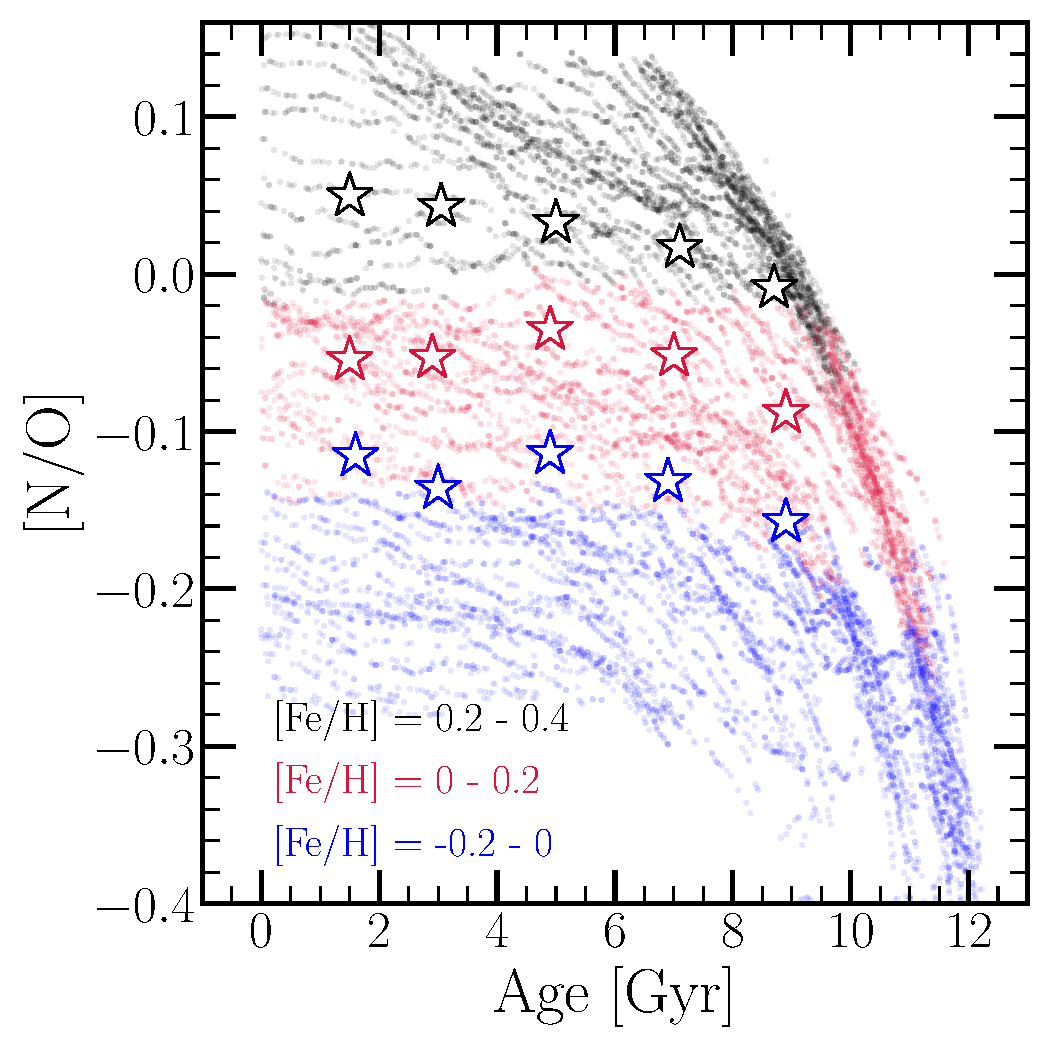
\includegraphics[scale = 0.3]{no_vs_age.pdf} 
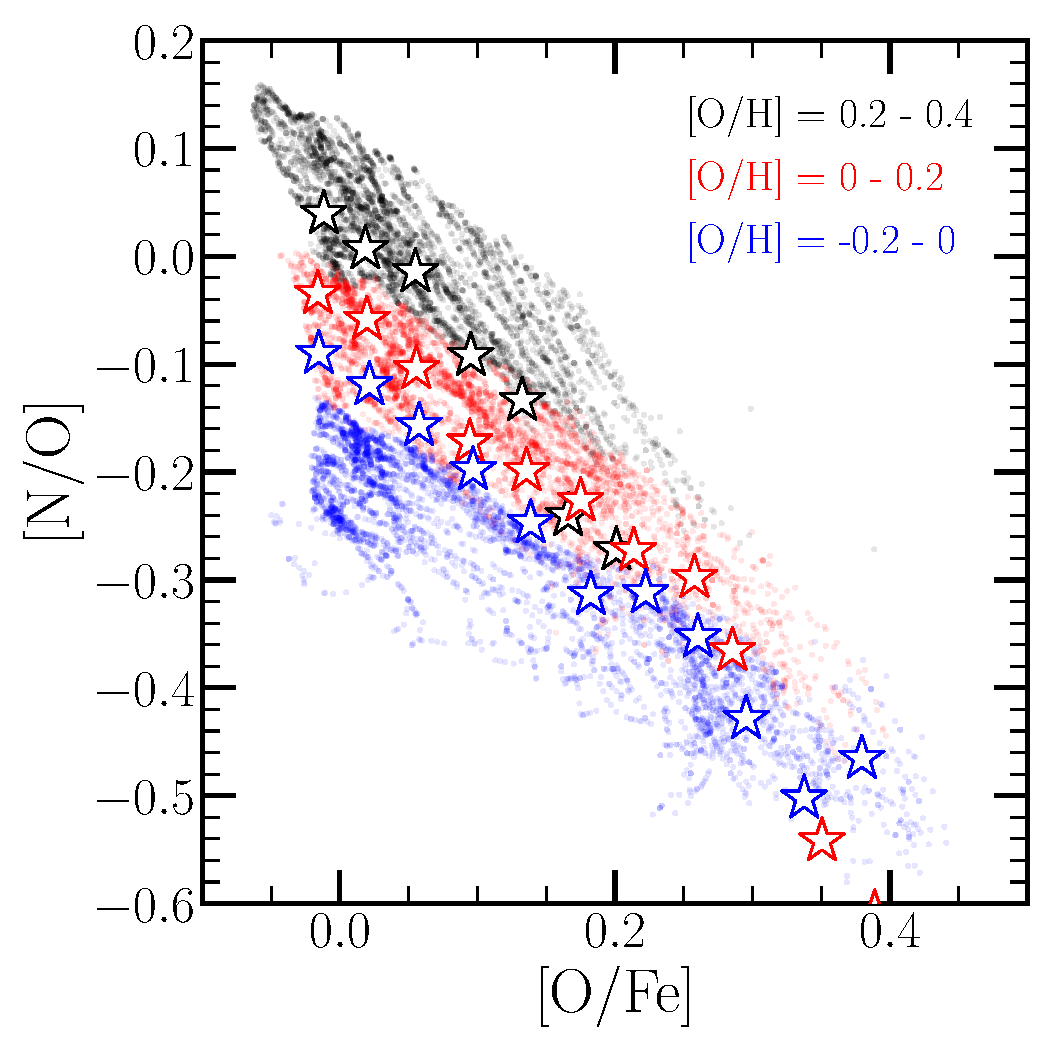
\includegraphics[scale = 0.3]{no_vs_ofe.pdf} 
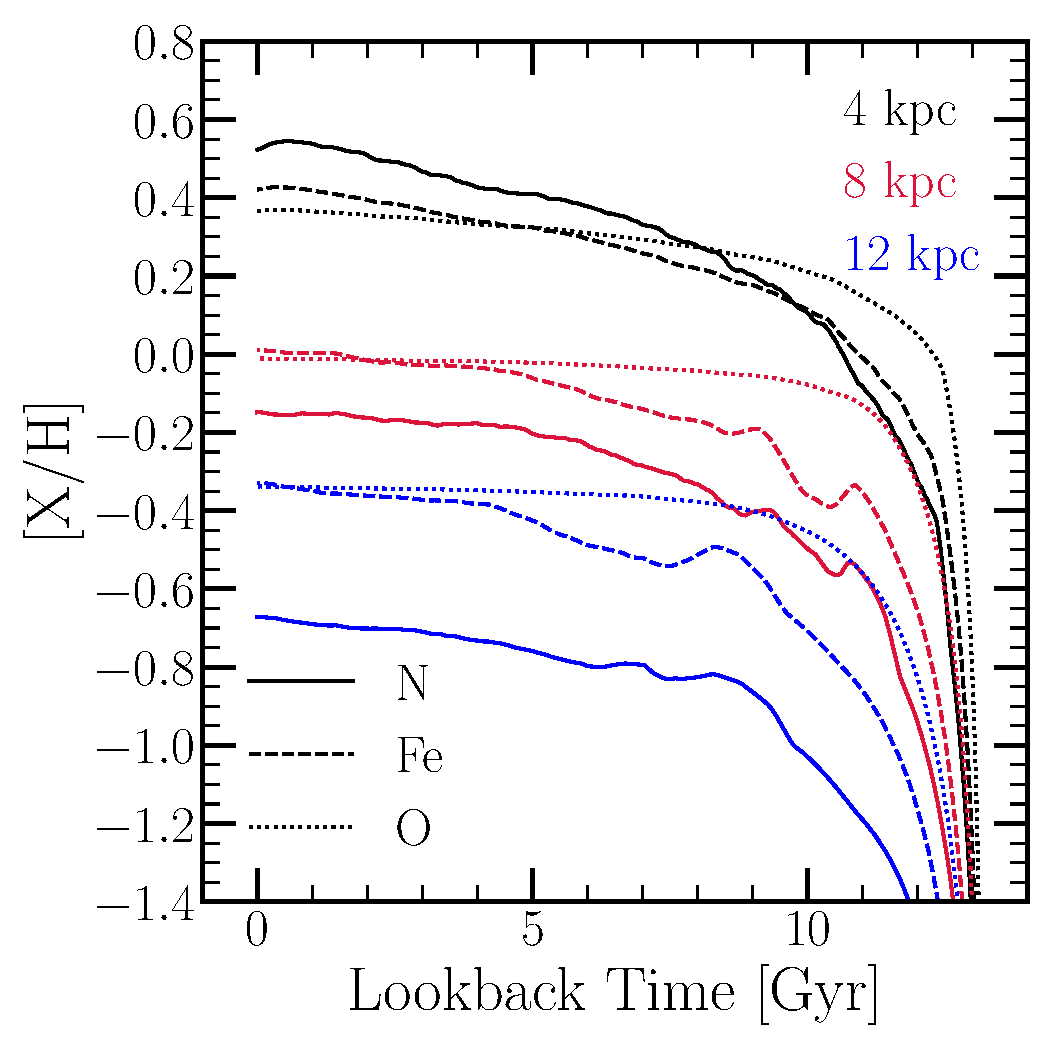
\includegraphics[scale = 0.3]{nh_feh_vs_lookback.pdf} 
\caption{
\textbf{Left}: [N/O] as a function of stellar age for 5000 stars randomly 
sampled from our model stellar populations in three bins of [Fe/H] (colored 
points). 
Stars quantify the median trend of [N/O] with age corrected for internal mixing 
in the same bins of [Fe/H] from the~\citet{Vincenzo2021} sample. 
\textbf{Middle}: The same as the left hand panel, instead showing [N/O] as a 
function of [O/Fe] in bins of [O/H]. 
\textbf{Right}: [N/O] (solid), [Fe/H] (dashed), and [O/H] (dotted) in the gas 
phase as a function of lookback time at~\rgal~= 4 (black), 8 (red), and 12 kpc 
(blue). 
} 
\label{fig:vincenzo_comp} 
\end{figure*} 

\subsection{The Stellar Abundances}  
\label{sec:results:vincenzo_comp} 

\begin{itemize} 
	\item Before comparing the predictions of GCE models to observational data, 
	it is essential that the N abundances be adjusted to account for internal 
	processes that alter the surface compositions of stars. 
	This is an important step to take before comparing GCE models to 
	observational data, because GCE models predict the birth abundances of 
	stars, and N abundances in evolved stars do not reflect their birth 
	abundance. 
	After the CNO cycle has processed much of the C and O nuclei into~\Nfourteen 
	during a star's main sequence lifetime, this N-rich material from the core 
	is mixed with the outer convective layers, increasing the N abundance in 
	the photosphere. 
	Using~\texttt{MESA} stellar evolution models~\citep{Paxton2011, Paxton2013, 
	Paxton2015, Paxton2018} with standard mixing prescriptions, 
	\citet{Vincenzo2021} developed a prescription to approximate the birth 
	abundances of C, N, and O and apply it to a sample of APOGEE/Kepler red 
	giants. 

	\item In the left hand panel of Fig.~\ref{fig:vincenzo_comp}, we compare 
	our model predictions to their [N/O] abundances with the ages taken 
	from~\citet{Miglio2021}. 
	The model correctly predicts that the [N/O]-age relation is relatively flat 
	in bins of [Fe/H]. 
	This is an important success of the model, because with uncorrected N 
	abundances, [N/O] vs. age exhibits a significant negative slope at fixed 
	[Fe/H] (see Fig. 7 of~\citealp{Vincenzo2021}). 
	Our model does, however, slightly underpredict [N/O] in the 
	[Fe/H] =~$-0.2 - 0$ bin. 
	In general, our model occupies a wider range in [N/O] at all ages than does 
	the~\citet{Vincenzo2021} measurements, suggesting that our yields scale 
	with metallicity slightly too strongly. 

	\item In the middle panel of Fig.~\ref{fig:vincenzo_comp}, we compare 
	our model predicted [N/O]-[O/Fe] relation to their calculations. 
	As in the left hand panel, our model predicted stellar populations occupy a 
	wider range of [N/O] than the data, but the agreement is otherwise good. 
	The model correctly predicts that [N/O] should increase with decreasing 
	[O/Fe] at all metallicities, and places the increase in [N/O] in the 
	highest [O/H] bin at approximately the correct value of [O/Fe]. 

	\item These results can generally be understood with the notion that 
	N and Fe abundances change on similar timescales in our model. 
	In the right hand panel of Fig.~\ref{fig:vincenzo_comp}, we show the time 
	evolution of [N/H], [Fe/H], and [O/H] in the gas phase at three different 
	radii. 
	[N/H] is more correlated with [Fe/H] than [O/H] at all radii, and the 
	relation persists up to lookback times of~$\sim$10 Gyr. 
	This arises largely because N and Fe are both produced in significant 
	quantities by delayed enrichment sources while O is produced almost 
	entirely on short timescales by CCSNe (see discussion 
	in~\S~\ref{sec:yields}). 
	As a consequence of its single dominant nucleosynthetic source, O reaches 
	an equilibrium abundance on much shorter timescales than elements like N 
	and Fe which have significant contributions from delayed 
	sources~\citep{Weinberg2017}; because of this, [O/H] is nearly 
	independent of lookback time as far back as~$\sim$10 Gyr ago while [N/H] 
	and [Fe/H] are not. 
	Therefore, a bin in [Fe/H] is also approximately a bin in [N/H], and with 
	[O/H] more or less constant, the [N/O]-age relation at fixed [Fe/H] is 
	relatively flat up to ages of~$\sim$10 Gyr. 
	The anti-correlation between [N/O] and [O/Fe] at fixed [O/H] is also a 
	direct consequence of the N-Fe correlation. 

	\item We thus conclude that when a viable model for the AGB star yields of 
	N is adopted, our GCE models are in good agreement with observed abundances 
	of N when corrected for internal mixing processes known to affect the 
	photospheric abundances in red giant stars. 
\end{itemize} 

\subsection{The Sources of Scatter in the [N/O]-[O/H] Relation} 
\label{sec:results:schaefer_comp} 

\begin{figure*} 
\centering 
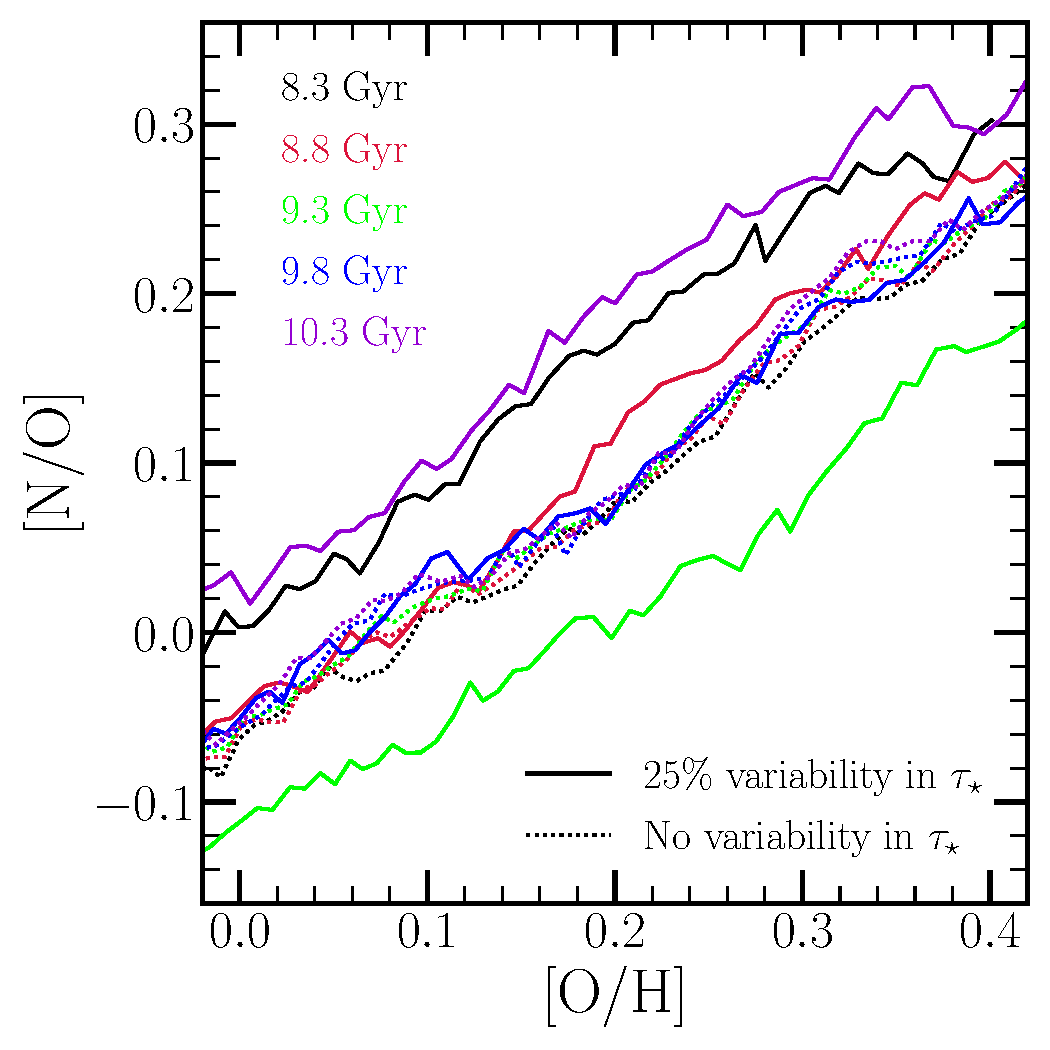
\includegraphics[scale = 0.31]{no_oh_sfevar.pdf} 
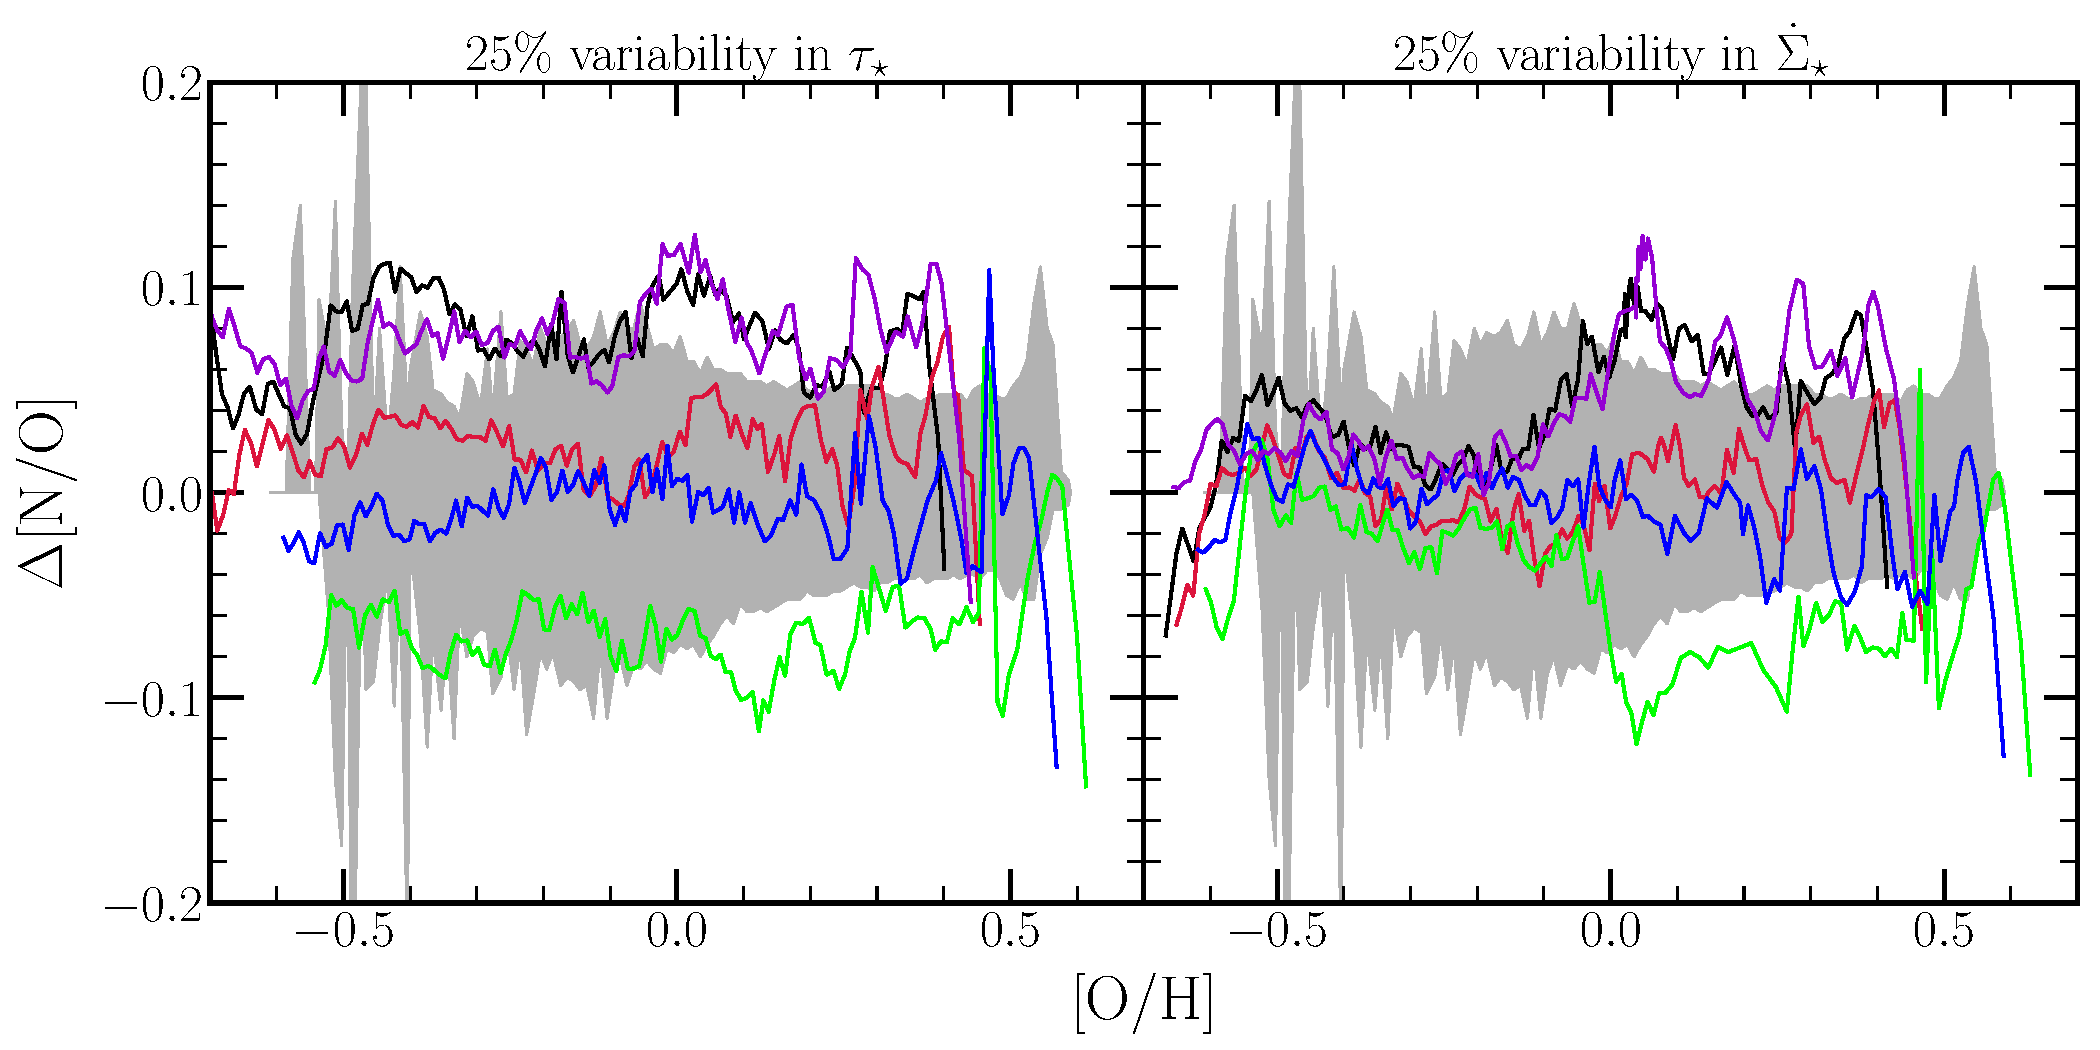
\includegraphics[scale = 0.33]{delta_no_schaefercomp.pdf} 
\caption{
\textbf{Left}: One cycle of oscillations in the [N/O]-[O/H] relation at high 
[O/H] induced by 25\% sinusoidal variability in~$\tau_\star$ (solid coloured 
lines). 
Dotted lines show the [N/O]-[O/H] relation at the same five snapshots in the 
fiducial model with no variability in~$\tau_\star$. 
The black dashed line shows the time evolution of the abundances in 
the~\rgal = 5 kpc ring, with the times of each of the five snapshots marked by 
a coloured point. 
\textbf{Middle and Right}: For the same five snapshots in the left hand panel, 
the deviation in [N/O] at fixed [O/H] relative to the fiducial model for the 
case with 25\% variability in~$\tau_\star$ (middle) and in~$\dot{\Sigma}_\star$ 
(right). 
The shaded regions in both panels quantify the width of the [N/O] distribution 
in~$10^{10.5} - 10^{11}$~\msun~galaxies in MaNGA taken 
from~\citet{Schaefer2020}. 
The median [N/O] is placed at~$\Delta$[N/O] = 0, and the lower (upper) envelope 
denotes the 16th (84th) percentile of the [N/O] distribution at a given [O/H]. 
} 
\label{fig:schaefer_comp} 
\end{figure*} 

\begin{itemize} 
	\item What is the dominant source of variance in the observed [N/O]-[O/H] 
	relation? 
	\citet{Schaefer2020} demonstrate that intrinsic scatter is driven by 
	variations in the local SFE - with slower star formation, more AGB stars 
	enrich the ISM by the time it reaches a given abundance, causing a higher 
	[N/O] at fixed [O/H]. 
	However, they did not rule out radial migration as another source of 
	scatter. 
	Can the radial migration of nucleosynthetic yields drive enough variation 
	in the gas-phase [N/O]-[O/H] relation to explain these results too? 
	Our models, taking into account the effects of radial migration on the 
	enrichment rates, are the ideal tool with which to answer this question. 

	\item We construct two additional models based on our fiducial model, one 
	in which the SFE exhibits 25\% sinusoidal variations in time, and the other 
	with the same 25\% variations in the SFR. 
	In these models, the SFE timescale~$\tau_\star$ and SFH~$\dot{\Sigma}_\star$ 
	are modified from the fiducial case in the following manner: 
	\begin{equation} 
	\tau_\star(\rgal, t) = \tau_{\star,\text{J21}}(\rgal, t)\left(1 + 0.25\sin 
	\left(\frac{2\pi t}{2\text{ Gyr}}\right)\right)
	\end{equation} 
	\begin{equation} 
	\dot{\Sigma}_\star(\rgal, t) = \dot{\Sigma}_{\star,\text{J21}}(\rgal, t) 
	\left(1 + 0.25\sin \left(\frac{2\pi t}{2\text{ Gyr}}\right)\right), 
	\end{equation} 
	where~$\tau_{\star,\text{J21}}$ and~$\dot{\Sigma}_{\star,\text{J21}}$ refer 
	to the SFE timescale and SFH in the fiducial model taken 
	from~\citet{Johnson2021}. 

	\item In a real galaxy, the variability in the SFE and the SFR are likely 
	non-sinusoidal and not with constant amplitude. 
	This, however, at least quantifies how much variation in [N/O] can be 
	expected by variations of a fixed amplitude in these quantities. 

	\item We find that 25\% variations in these quantities generally induce 
	larger variability than does stellar migration. 
	In the left hand panel of Fig.~\ref{fig:schaefer_comp}, we plot the 
	predicted gas-phase [N/O]-[O/H] relation at high [O/H] for five snapshots 
	covering one cycle of the fluctuations induced by variability 
	in~$\tau_\star$. 
	The model with no sinusoidal oscillations in~$\tau_\star$ predicts the 
	relation to be nearly constant over this time interval, whereas the model 
	with them predicts a~$\sim$0.15-dex dynamic range. 

	\item Such behavior is driven by the constant tug-of-war between dilution 
	and re-enrichment associated with oscillations in~$\tau_\star$. 
	In this model,~$\dot{\Sigma}_\star$ is the same as it was 
	in~\citet{Johnson2021}, so it is not~$\dot{\Sigma}_\star$ which is 
	fluctuating, but rather~$\Sigma_\text{gas}$. 
	When the gas supply increases, the ISM becomes diluted, decreasing [O/H]. 
	Because the AGB star yields of N with our fiducial~\cristallo~model are 
	roughly linear with metallicity, the decrease in the N abundance due to the 
	now lowered yields are in direct proportion to the amount of dilution. 
	As a result, [N/O] is only marginally affected by the fluctuations in the 
	overall abundance. 
	The variations in the [N/O]-[O/H] relation that the model predicts are 
	therefore more of a consequence of variability in [O/H] than in [N/O]. 
	We demonstrate this with the black dashed line in the left hand panel of 
	Fig.~\ref{fig:schaefer_comp}, which traces out the evolution of the 
	abundances at~\rgal~= 5 kpc over the same time interval. 
	In general, [N/O] is affected only at the~$\sim$0.05-dex level while 
	[O/H] varies with an amplitude of~$\sim$0.25-dex. 
	As the gas supply falls off, enrichment proceeds in a gas-starved ISM, 
	which increases [O/H] once more, but [N/O] to a lesser extent for similar 
	reasons, and the cycle repeats itself. 

	\item When~$\dot{\Sigma}_\star$ varies,~$\Sigma_\text{gas}$ and 
	consequently the abundances vary instead at a value of~$\tau_\star$ that 
	varies only as much as the adopted~$\dot{\Sigma}_\star - \Sigma_\text{gas}$ 
	relation from~\citet{Johnson2021} dictates it should (see discussion in 
	\S~\ref{sec:methods}), with no additional variations in time. 

	\item In the middle and right hand panels of Fig.~\ref{fig:schaefer_comp}, 
	we plot the difference in [N/O] at fixed [O/H] between the fiducial model 
	and those with variability as a function of [O/H] (i.e. the vertical 
	offset between the solid and dotted curves in the left hand panel). 
	Both scenarios produce offsets in [N/O] at high [O/H] (which as discussed 
	above are truly offsets in [O/H] at fixed [N/O]), but the model with 
	variations in~$\dot{\Sigma}_\star$ does not predict any significant 
	fluctuations in the abundances at [O/H]~$\lesssim -0.2$. 
	This is a consequence of the mathematical form of~$\tau_{\star,\text{J21}}$ 
	(see discussion in~\S~\ref{sec:methods}) and the fact that we 
	have run these models in star formation mode with~\vice. 
	The low [O/H] end of the relation comes from the outer Galaxy at lower 
	$\Sigma_\text{gas}$ than the inner regions at higher [O/H], and the surface 
	densities are in the region where~$\Sigma_\text{gas} 
	\sim \dot{\Sigma}_\star^{3.6}$. 
	However, in these models,~$\dot{\Sigma}_\star$ is fixed, meaning that it is 
	not a strong function of~$\Sigma_\text{gas}$ - rather~$\Sigma_\text{gas}$ 
	is only a weak function of~$\dot{\Sigma}_\star$. 
	25\% oscillations in~$\dot{\Sigma}_\star$ therefore have little impact on 
	the ISM gas supply, and as a consequence the impact on abundances is 
	minimal. 
	At smaller~\rgal~(i.e. higher [O/H]),~$\Sigma_\text{gas}$ varies more 
	strongly with~$\dot{\Sigma}_\star$, and thus there is a stronger effect on 
	the abundances there. 
	In the model with oscillations in~$\tau_\star$,~$\Sigma_\text{gas}$ always 
	varies with a~25\% amplitude, so the oscillations are seen at all 
	abundances. 
	If we were to adopt an alternate form of the~$\dot{\Sigma}_\star - 
	\Sigma_\text{gas}$ relation in these models, such as a purely linear or 
	single power-law formalism, then the impact on abundance would be seen at 
	all [O/H] when~$\dot{\Sigma}_\star$ oscillates. 
	Alternatively, we expect a similar result if we were to run an equivalent 
	model in infall mode (i.e. specifying the infall history and initial gas 
	supply rather than the star formation history). 

	\item The shaded regions in the left and middle panels of 
	Fig.~\ref{fig:schaefer_comp} quantify the scatter in the gas-phase 
	[N/O]-[O/H] relation inferred observationally by~\citet{Schaefer2020}. 
	Using data from Mapping nearby Galaxies at Apache Point Observatory 
	(MaNGA;~\citealp{Bundy2015}), an integral field unit survey, they measure 
	N and O abundances in 709,541 spaxels across 6,507 unique galaxies spanning 
	a stellar mass range from~$10^9 - 10^{11}$~\msun. 
	Since our model is appropriate for Milky Way mass galaxies, we focus our 
	comparison on the~$M_\star = 10^{10.5} - 10^{11}$~\msun~range, which cuts 
	our sample to 197,787 individual N and O measurements from the MaNGA IFU 
	spaxels. 
	In narrow bins of [O/H], we then compute the median [N/O] as well as the 
	16th and 84th percentiles of the [N/O] distribution. 
	Placing the median [N/O] at~$\Delta$[N/O] = 0, the shaded regions above and 
	below 0 in Fig.~\ref{fig:schaefer_comp} denote the difference between the 
	16th and 84th percentile of the distribution in each bin. 

	\item Our models with 25\% sinusoidal oscillations in~$\dot{\Sigma}_\star$ 
	and~$\tau_\star$ produce deviations in [N/O] at fixed [O/H] that are 
	comparable to the width of the distribution measured observationally. 
	Stellar migration, on the other hand, induces only small variations, as can 
	be seen in the left-hand panel of Fig.~\ref{fig:schaefer_comp}. 
	This traces back to the timescales of N production from single stellar 
	populations (see Fig.~\ref{fig:no_oh_predictions} and discussion 
	in~\S~\ref{sec:results:fiducial}): most N production occurs quickly 
	following a stellar population's formation ($\sim$few hundred Myr), meaning 
	that most stars will not migrate far from their birth radius by the time 
	they produce their N, and the resulting impact on the gas phase abundances 
	is minimal. 

	\item In general, galaxies will not have perfectly sinusoidal variations in 
	their SFR or SFE, and they will also not be of a constant amplitude. 
	Nonetheless, these models clearly demonstrate that the expected differences 
	in N and O abundances in the gas phase is larger than that caused by radial 
	migration as conjectured by~\citet{Schaefer2020}. 
	Such variations will present as scatter in the gas phase abundances by 
	observing many galaxies at different phases and with different amplitudes 
	in their variability, which may be much more complicated that the sinusoids 
	modeled here. 
\end{itemize} 

% \begin{figure*} 
% \centering 
% 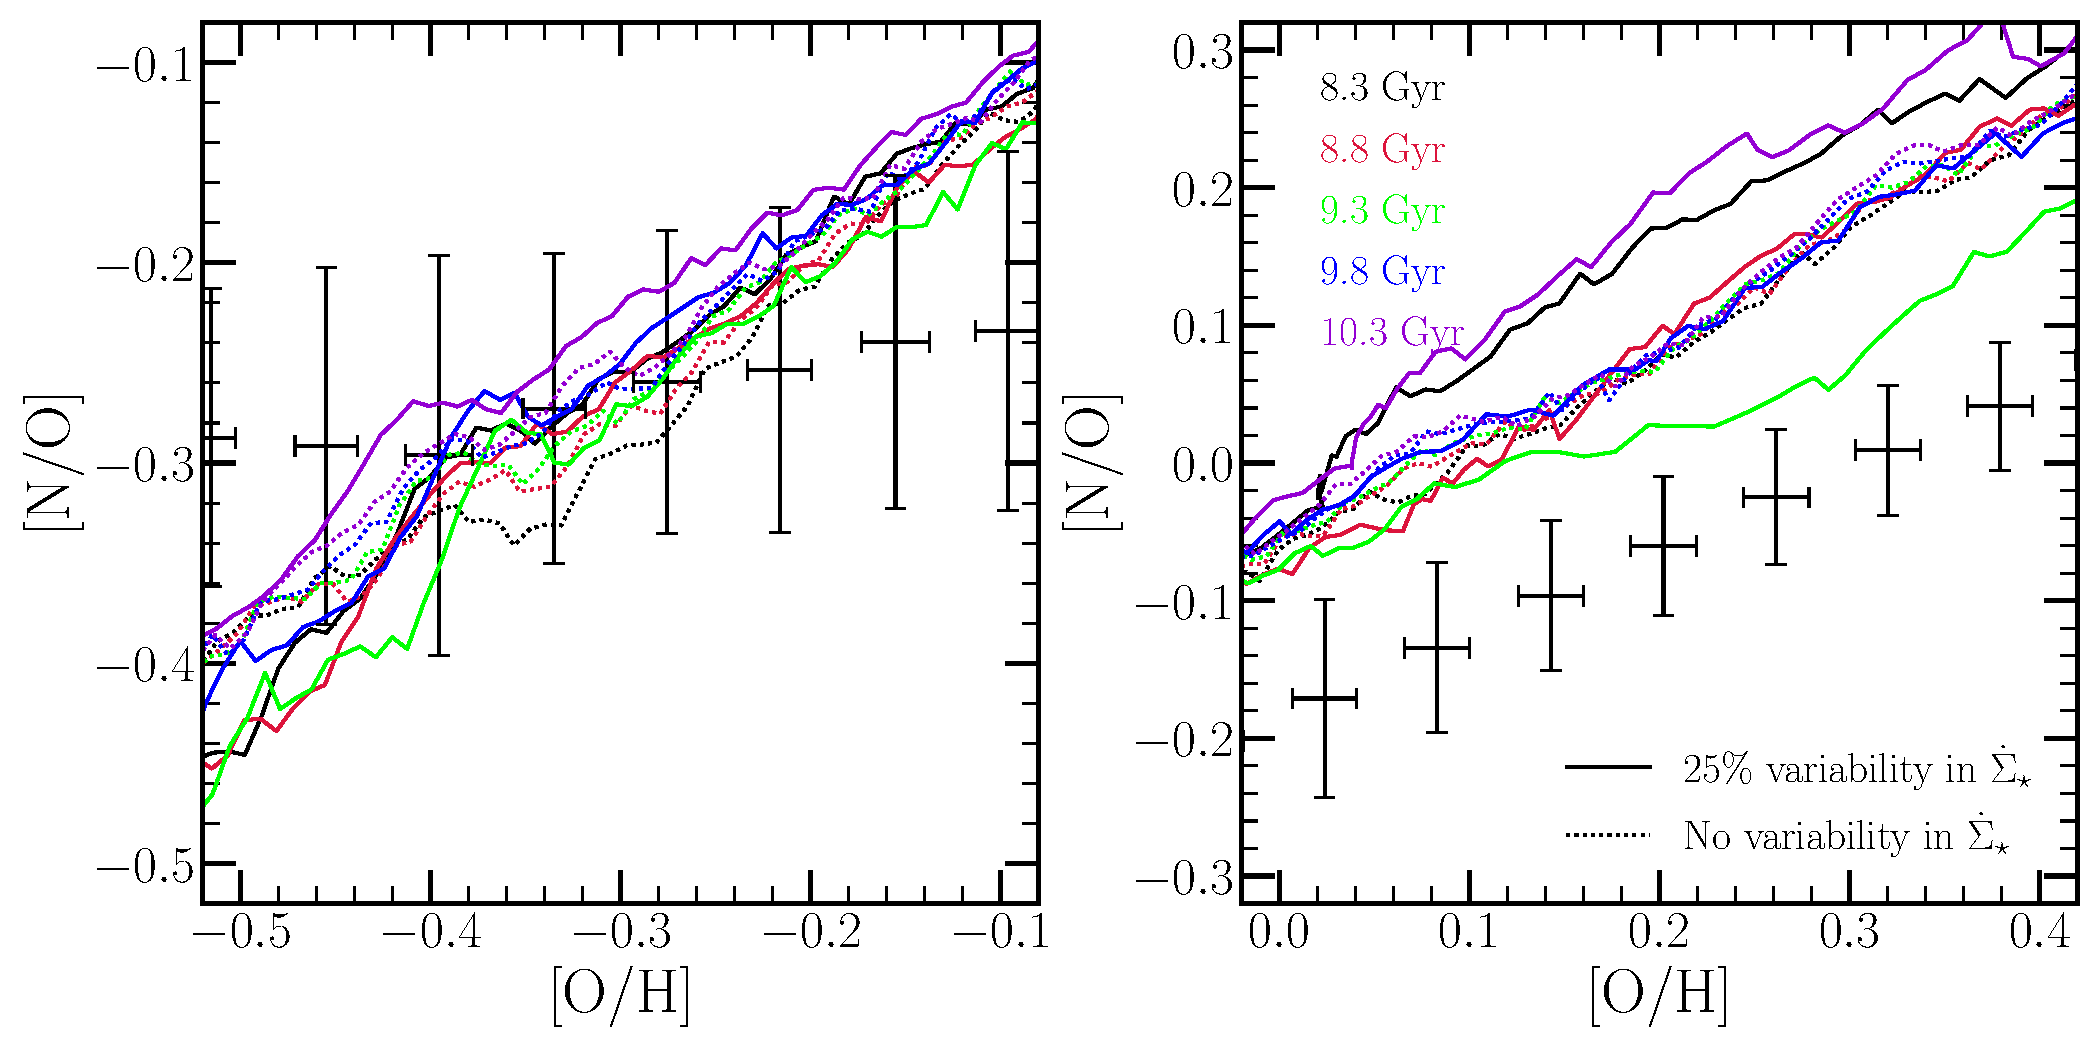
\includegraphics[scale = 0.45]{no_oh_modsfr.pdf} 
% 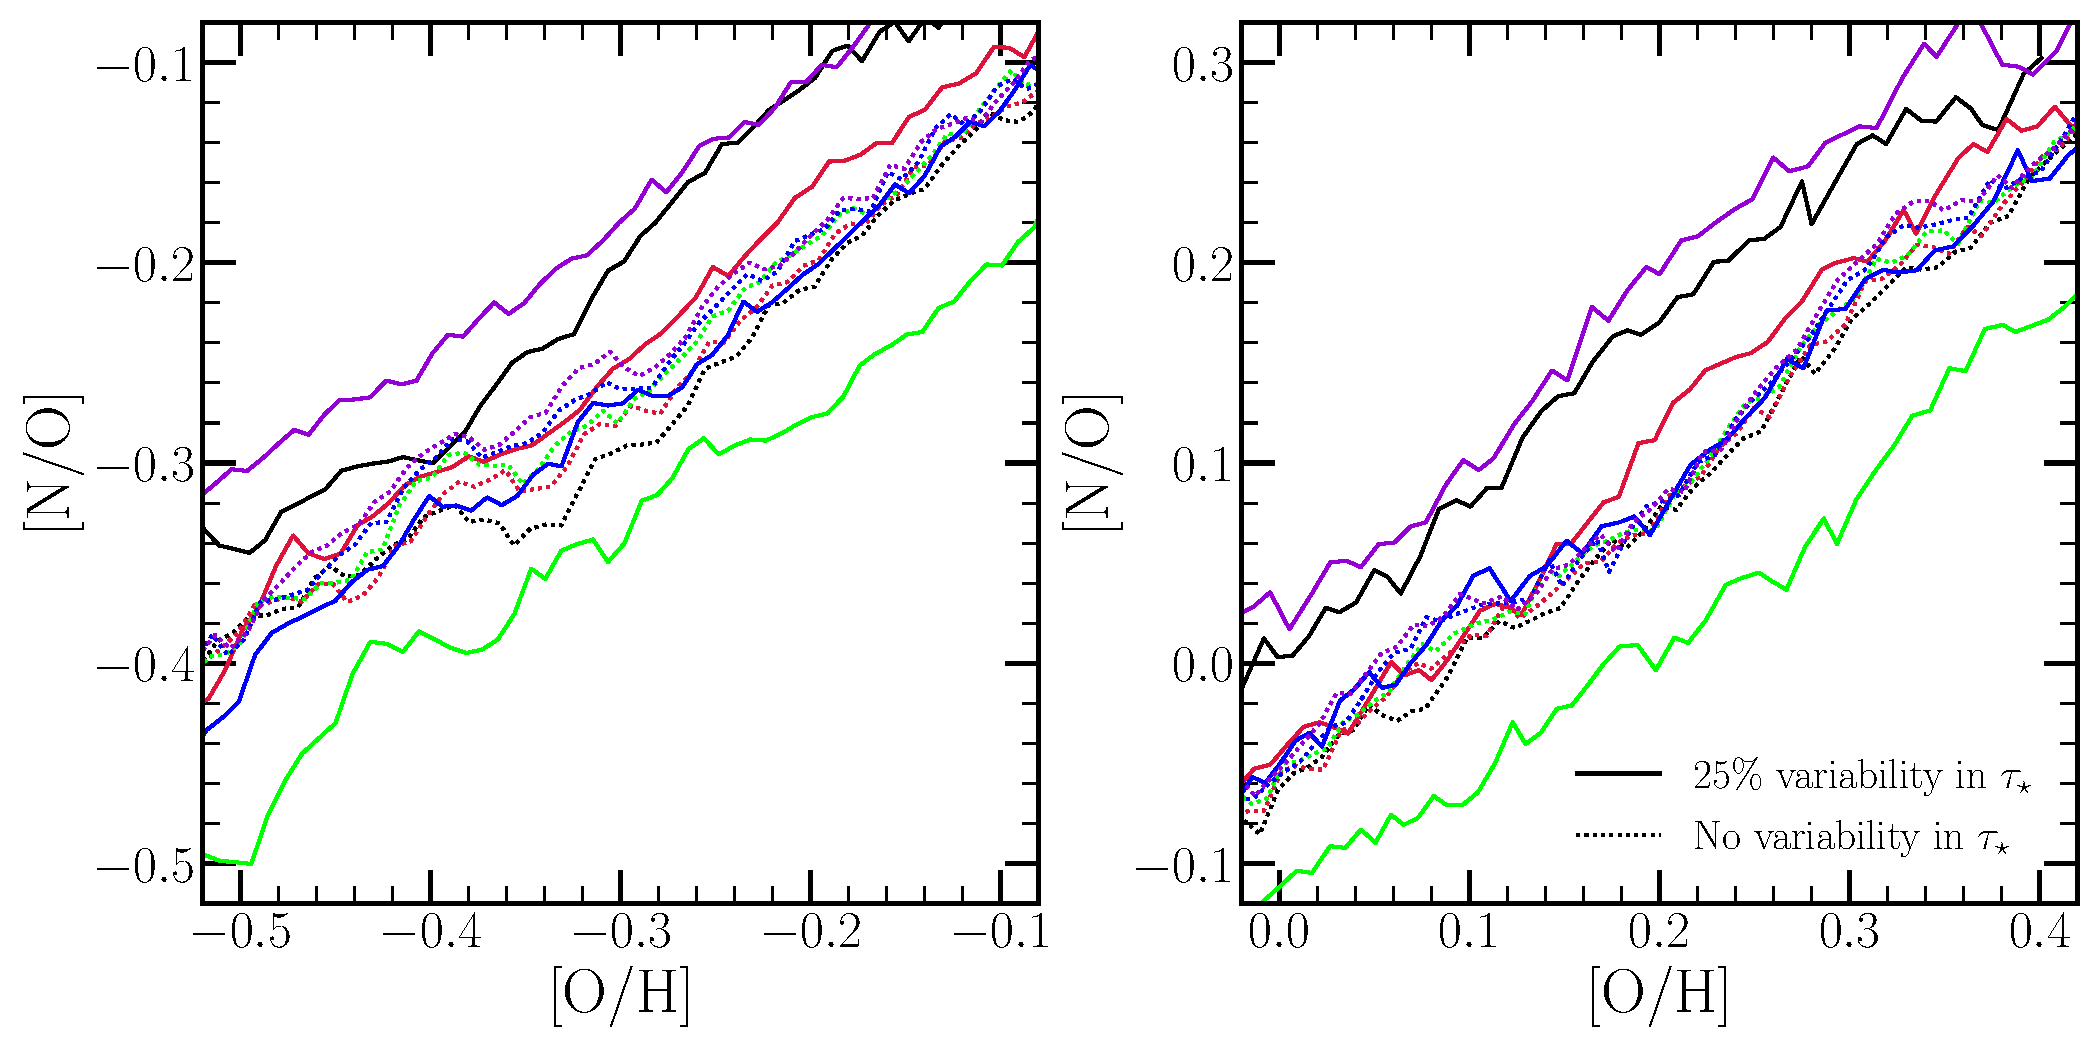
\includegraphics[scale = 0.45]{no_oh_modsfe.pdf} 
% \caption{
% One cycle of variability in the gas-phase [N/O]-[O/H] relation at low [O/H] 
% (left) and high [O/H] (right) induced by 25\% sinusoidal variations in the SFR 
% (top) and in the SFE (bottom). 
% Solid lines denote the models with some source of variability, and dotted lines 
% denote the fiducial model with no variability; all models take into account the 
% effects of stellar migration. 
% } 
% \label{fig:no_oh_mods} 
% \end{figure*} 

\end{document} 

